\documentclass{article}
% Author: Luan Leal
% Last update: 2024-12-03

% ----------------------------

% ----------------------------   IMPORTS   ----------------------------
\usepackage{amssymb, amsthm, amsmath, geometry, siunitx, caption, float, graphicx}
\usepackage{enumitem}
\usepackage[utf8]{inputenc}
\usepackage[onehalfspacing]{setspaceenhanced}
\usepackage[brazil]{babel} % Adaptação ao pt-br
\usepackage{hyperref} % Usado para inserir links
\usepackage[capitalize, brazilian, noabbrev]{cleveref} % Referência adaptada ao pt-br
\usepackage{subcaption}
\usepackage{makecell}
\usepackage[num,overcite]{abntex2cite}

% ----------------------------   LAYOUT   ----------------------------
\citebrackets[]
\geometry{a4paper, lmargin=3cm, tmargin=3cm, rmargin=2cm, bmargin=2cm}
\onehalfspacing
%\setlength{\parindent}{45pt}
\sisetup{output-decimal-marker = {,}}

% ----------------------------  THEOREMS  ----------------------------
% -Ambiente de definição
\theoremstyle{definition}
\newtheorem{dfn}{Definição}[section]

% -Ambiente de observação
\theoremstyle{remark}
\newtheorem{obs}{Observação}

% -Ambiente de lema
\theoremstyle{definition}
\newtheorem{lema}{Lema}

% -Ambiente de exemplo
\theoremstyle{definition}
\newtheorem{xp}{Exemplo}[section]

% -Ambiente de proposição
\newtheorem{prop}{Proposição}

% -Ambiente de teorema e demonstração
\theoremstyle{plain}
\newtheorem{thm}{Teorema}
\theoremstyle{remark}
\newtheorem*{dms}{Demonstração}

% -Ambiente de exercício e resolução
\theoremstyle{definition}
\newtheorem{xcs}{Exercício}
\theoremstyle{remark}
\newtheorem*{rsl}{Resolução}

% ----------------------------  COMMANDS  ----------------------------
%\newcommand{\RR}{\mathbb{R}} % \mathbb{R} = \RR
%\newcommand{\ZZ}{\mathbb{Z}} % \mathbb{Z} = \ZZ

\author{Matheus Justino; Matheus Queiroz; Micael Baruch; Luan Leal}
\title{0-ésima Prova de Química II}

\begin{document}
\maketitle

    \textbf{Utilize caso achar necessário \(R = \qty{8,3145}{J\ K^{-1} mol^{-1}}, \
    R = \qty{0,082057}{L\ atm\ K^{-1} mol^{-1}}, \ 
    R = \qty{82,05745}{cm^3\ atm\ K^{-1} mol^{-1}}, \
    R = \qty{1,897}{cal\ K^{-1} mol^{-1}}\).
    Justifique sua resposta e mostre as etapas de cálculo. Não esqueça das
    unidades!}
    
    \textbf{(1)} O fluoreto de nitrila (\ce{NO2F}) é um gás incolor e um agente oxidante forte empregado como agente fluoretante. É uma espécie molecular (não iônica) e possui estrutura planar. O estudo de suas propriedades termodinâmicas e de sua formação foi realizado em 1962 por E. Tschuikow-Row\textsuperscript{1}, o qual verificou o mecanismo de formação e sua dependência com a temperatura através de espectroscopias vibracionais (Raman e IV).\\

A reação global observada foi:
\begin{align*}
    2\,\ce{NO2}(g) + \ce{F2}(g) \rightarrow 2\,\ce{NO2F}(g)
\end{align*}

 Essa reação, no entanto, apresentou um mecanismo complexo cuja lei de velocidade é dada por:
\begin{align*}
    v = k[\ce{NO2}][\ce{F2}]
\end{align*}

e o estudo de suas propriedades termodinâmicas apresentou variação da constante de equilíbrio ($K_{\text{eq}}$) em função da temperatura na etapa determinante (etapa lenta), conforme (ln$K_{\text{eq}}$) na tabela abaixo:

\begin{center}
\begin{tabular}{|c|c|c|c|c|c|c|c|c|c|}
\hline
\textbf{T / K} & 200 & 300 & 400 & 500 & 600 & 700 & 800 & 900 & 1000 \\
\hline
\textbf{ln $K_{\text{eq}}$} & 7,55 & 14,43 & 17,84 & 19,85 & 21,16 & 22,08 & 22,72 & 23,28 & 23,67 \\
\hline
\end{tabular}
\end{center}

\bigskip

Com todas essas informações em mãos:\\

\textbf{a)} Proponha o mecanismo de reação para a formação do \ce{NO2F} e explicite a etapa determinante;\\

\textbf{Resposta:} 

Para propor o mecanismo de reação para a formação do \ce{NO2F}, partimos da equação global observada:
\begin{align*}
2\ \ce{NO2}(g) + \ce{F2}(g) \rightarrow 2\ \ce{NO2F}(g)
\end{align*}

Embora a reação pareça simples, estudos experimentais revelaram que ela ocorre por um mecanismo mais complexo, sendo a sua velocidade regida pela expressão:
\begin{align*}
v = k[\ce{NO2}][\ce{F2}]
\end{align*}

Essa lei de velocidade indica que a etapa determinante (ou etapa lenta) do processo envolve uma colisão entre uma molécula de \ce{NO2} e uma molécula de \ce{F2}, ou seja, é uma etapa bimolecular. A partir disso, propõe-se o seguinte mecanismo:

\textit{Etapa lenta (determinante):}
\begin{align*}
\ce{NO2 + F2 -> NO2F + F}
\end{align*}

\textit{Etapa rápida:}
\begin{align*}
\ce{F + NO2 -> NO2F}
\end{align*}

Somando as etapas:
\begin{align*}
&\ce{NO2 + F2 -> NO2F + F} \hspace{1.0cm} \text{(etapa lenta)}\\
&\ce{F + NO2 -> NO2F} \hspace{1.8cm} \text{(etapa rápida)}\\
\midrule %Alguém sabe ajeitar essa linha maldita?
&\ce{2NO2 + F2 -> 2NO2F} \hspace{1.2cm} \text{(equação global)}
\end{align*}

Dessa forma, o mecanismo é consistente tanto com a estequiometria global quanto com a lei de velocidade observada experimentalmente, e evidencia que a etapa determinante é a formação do intermediário a partir de \ce{NO2} e \ce{F2}.

\vspace{0.4cm}

\textbf{b)} Proponha a estrutura do complexo ativado para essa reação bimolecular;\\

\textbf{Resposta:} 

Para representar a estrutura do complexo ativado dessa reação bimolecular, é necessário considerar que, durante a colisão entre \ce{NO2} e \ce{F2}, ocorre uma reorganização eletrônica na qual uma das ligações F–F começa a se romper ao mesmo tempo que uma nova ligação N–F começa a se formar. Esse estado de transição pode ser representado por uma estrutura em que os átomos ainda não estão completamente ligados, caracterizando o chamado “complexo ativado” ou “estado de transição”.

A estrutura pode ser descrita como:
\begin{align*}
\ce{[NO2 \cdots F \cdots F]^{\ddagger}}
\end{align*}

Nesse intermediário, o flúor mais próximo do nitrogênio do \ce{NO2} apresenta uma ligação parcialmente formada com o N, enquanto a ligação F–F encontra-se parcialmente rompida. Além disso, a geometria ao redor do nitrogênio provavelmente se torna levemente distorcida em relação ao plano original da molécula, dada a reorganização eletrônica em curso. Essa estrutura representa o ponto de maior energia no caminho da reação, ou seja, o topo da barreira energética que os reagentes devem superar para formar os produtos.

\vspace{0.4cm}

\textbf{c)} Apresente a curva de energia potencial de formação do \ce{NO2F}, apontando a região da curva onde ocorre a formação do complexo ativado. De acordo com suas observações, essa reação é endotérmica ou exotérmica? Explique com o devido formalismo.\\

\textbf{Resposta:} 

Com base nos dados fornecidos sobre a constante de equilíbrio (\(K_\text{eq}\)) da etapa determinante em diferentes temperaturas, é possível analisar a natureza energética do processo e determinar se a reação é endotérmica ou exotérmica. A tabela mostra que o valor de \(\ln(K_\text{eq})\) aumenta com o aumento da temperatura, o que implica que a constante de equilíbrio também cresce. Isso pode ser interpretado por meio da equação de Van’t Hoff:
\begin{align*}
\ln(K_\text{eq}) = -\frac{\Delta H^\circ}{R} \cdot \frac{1}{T} + \frac{\Delta S^\circ}{R}
\end{align*}

Esta equação lineariza a relação entre \(\ln(K_\text{eq})\) e o inverso da temperatura \(1/T\). Uma análise preliminar da tabela de dados já indicava que o valor de \(\ln(K_\text{eq})\) aumenta com o aumento da temperatura. Esse comportamento é característico de reações endotérmicas, pois o equilíbrio se desloca para a direita (formação de produtos) com o aumento da temperatura, o que implica um \(\Delta H^\circ\) positivo.

Para quantificar essa variação de entalpia, realizamos uma regressão linear dos dados de \(\ln(K_\text{eq})\) em função de \(1/T\). O gráfico resultante dessa regressão está apresentado na (\cref{fig:vant})

\begin{figure}[H]
\centering
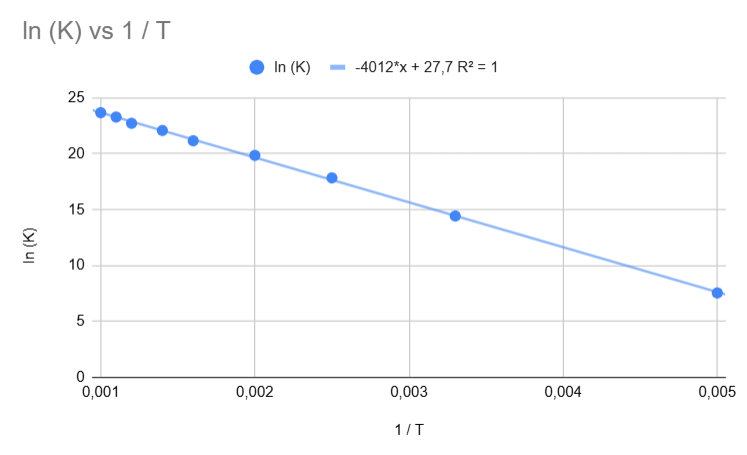
\includegraphics[width=0.7\linewidth]{fig/regressao.png}
\caption{Gráfico de \(\ln(K_\text{eq})\) versus \(1/T\) para a etapa determinante, com a linha de regressão linear.}
\label{fig:vant}
\end{figure}

A partir da regressão linear, obtivemos a equação da reta que descreve o comportamento dos dados:
\begin{align*}
\ln(K_\text{eq}) = -4012 \text{ K} + 27,7
\end{align*}

Comparando esta equação com a forma linear da Equação de Van't Hoff \(y = mx + b\), identifica-se diretamente o coeficiente angular da reta como \(m = -4012 \text{ K}\). Pela Equação de Van't Hoff, sabemos que o coeficiente angular é \(m = -\frac{\Delta H^\circ}{R}\). Portanto, podemos rearranjar a equação para calcular \(\Delta H^\circ\):
\begin{align*}
    \Delta H^\circ = -m \times R
\end{align*}

Substituindo os valores conhecidos do coeficiente angular e da constante dos gases ideal \(R = 8.314 \frac{J}{mol.K}\):
\begin{align*}
& \Delta H^\circ = -(-4012 \text{ K}) \times (8.314 \text{ J} \cdot \text{mol}^{-1} \cdot \text{K}^{-1}) \\
& \Delta H^\circ = 4012 \times 8.314 \text{ J} \cdot \text{mol}^{-1} \\
& \Delta H^\circ = 33355.768 \text{ J} \cdot \text{mol}^{-1}
\end{align*}

Convertendo o valor para quilojoules por mol \(kJ/mol\), para maior clareza e padronização em termodinâmica:
\begin{align*}
    \Delta H^\circ \approx +33.35 \text{ kJ} \cdot \text{mol}^{-1}
\end{align*}

O resultado obtido, $\Delta H^\circ = +33.35 \text{ kJ} \cdot \text{mol}^{-1}$, indica que a variação de entalpia para a etapa determinante da reação de formação do $\ce{NO2F}$ é positiva, ou seja, que a etapa determinante da reação de formação do $\ce{NO2F}$ é endotérmica. Isso significa que essa etapa absorve energia do ambiente para prosseguir.

Essa característica endotérmica é ilustrada no diagrama de energia potencial em função da coordenada de reação (\cref{diagrama}). No diagrama, os reagentes se encontram em um patamar energético inicial. À medida que a reação prossegue, a energia do sistema aumenta até atingir um máximo, correspondente ao complexo ativado — o ponto mais instável e de maior energia do processo. Após ultrapassada essa barreira, a energia diminui com a formação dos produtos.

    \begin{figure}[H]
        \centering
        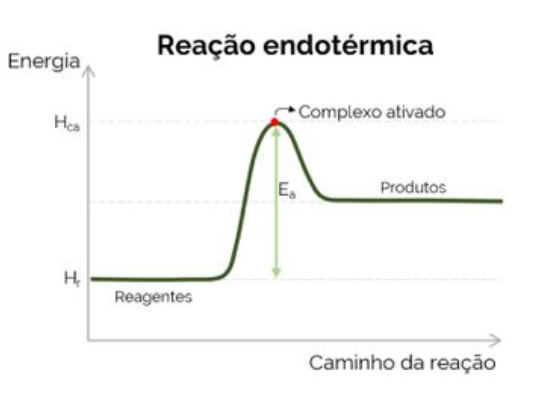
\includegraphics[width=0.35\linewidth]{fig/grafico.png}
        \caption{curva de energia potencial de formação do \ce{NO2F}}
        \label{diagrama}
    \end{figure}

Como a energia dos produtos é maior do que a dos reagentes, a variação de entalpia total da reação (\(\Delta H\)) é positiva, reforçando que o processo é endotérmico. A energia de ativação (\(E_\text{a}\)) corresponde à diferença entre os reagentes e o complexo ativado, e sua magnitude está relacionada à taxa com que a reação ocorre: quanto maior a \(E_\text{a}\), mais lenta é a reação, justificando a sua presença como etapa determinante.

Portanto, a partir da análise dos dados de equilíbrio via regressão linear pela Equação de Van't Hoff e da representação no diagrama de energia, conclui-se que a formação do \ce{NO2F} apresenta uma etapa lenta que é endotérmica, com formação de um complexo ativado de alta energia, e que a reação global ocorre mediante superação dessa barreira, em consonância com o modelo energético das reações químicas e o formalismo termodinâmico.

    \begin{xcs}
    A equação \( P = \frac{RT}{V_m - b} \) é algumas vezes utilizada para
    descrever o comportamento de gases reais. 
    \begin{enumerate}[label=\alph*.]
        \item É possível liquefazer gases que seguem essa equação? Justifique
            seu raciocínio. Sugestão: considere a similaridade da equação com a
            equação de van der Waals. 
    \end{enumerate}
\end{xcs}
\begin{rsl}
    Primeiro, avaliamos a definição de líquido: um fluído constituído de partículas
    globalmente desorganizadas que ocupam volume máximo. Dado
\end{rsl}

    \begin{xcs}
    A equação \( P = \frac{RT}{V_m - b} \) é algumas vezes utilizada para
    descrever o comportamento de gases reais. 
    \begin{enumerate}[label=\alph*.]
        \item[b.] Discuta as condições que uma equação deve satisfazer para ser
            empregada como uma equação de estado de um gás real e verifique se a
            equação acima satisfaz tais condições (ou seja, demonstre
            matematicamente). 
    \end{enumerate}
\end{xcs}
\begin{rsl}
    
\end{rsl}

    \begin{xcs}
    A \qty{273}{K}, o argônio tem os seguintes coeficientes do virial: 
    B = \qty{-21,7}{cm^3 mol^{-1}} e C = \qty{1200}{cm^6 mol^{-2}}.
    Admitindo que a lei dos gases perfeitos seja
    suficientemente exata para estimar o segundo e terceiro termos da expansão
    (ou seja, use a lei dos gases perfeitos em caso de necessidade): 
    \begin{enumerate}[label=\alph*.]
        \item calcule o fator de compressibilidade do argônio a 100 atm e 273 K.
            Sugestão: Obtenha uma expressão para Z em função de P com B, C e T
            constantes. 
    \end{enumerate}
\end{xcs}
\begin{rsl}
    %TODO: Parece que falta tudo? Que coisa...
    \begin{align*}
        Z = (1 + \frac{-21,7 \cdot 100}{273 \cdot 82,057} + 
        \frac{1200 \cdot 100^2}{273^2 \cdot 82,057^2}) 
        = 0,927
    \end{align*}
\end{rsl}

    \begin{xcs}
    A \qty{273}{K}, o argônio tem os seguintes coeficientes do virial: 
    B = \qty{-21,7}{cm^3 mol^{-1}} e C = \qty{1200}{cm^6 mol^{-2}}.
    Admitindo que a lei dos gases perfeitos seja
    suficientemente exata para estimar o segundo e terceiro termos da expansão
    (ou seja, use a lei dos gases perfeitos em caso de necessidade): 
    \begin{enumerate}[label=\alph*.]
        \item[b.] Explique como o fator de compressibilidade Z varia com a
            temperatura. Faça um esboço indicando o comportamento de Z acima e
            abaixo da temperatura de Boyle (T\(_B\)), identificando também essa
            temperatura no esboço. 
    \end{enumerate}
\end{xcs}
\begin{rsl}
    %TODO: Falta tudo...
    
\end{rsl}


\end{document}
